% orientation_pipeline -- schematic of the Spectral Surface Generation pipeline
% for an arbitrary Hamiltonian, no subset-sum content.
%   (H,|psi>) --acquire--> {G(t_k)} --classical reconstruct--> Z_tau(s)
%     --derivatives--> {mu_tau, sigma^2_tau, kappa_m, ratios, staircase}
% Lower strip: one generic spectrum viewed at several locations s / resolutions
% 1/sqrt(tau), and the supported (s,tau) region bounded by acquisition time + noise.
% Schematic, no data dependency. Palette matches eigenengine.sty.
\documentclass[tikz,border=4pt]{standalone}
\usepackage{amsmath}
\usepackage{bm}
\usetikzlibrary{arrows.meta,positioning,backgrounds,fit,calc}

\definecolor{ink}{HTML}{1A1A2E}
\definecolor{phys}{HTML}{2C6FAD}
\definecolor{acc}{HTML}{C0392B}
\definecolor{faint}{HTML}{9AA5B1}
\definecolor{physbg}{HTML}{EAF1F8}
\definecolor{inkbg}{HTML}{F2F3F5}

\begin{document}
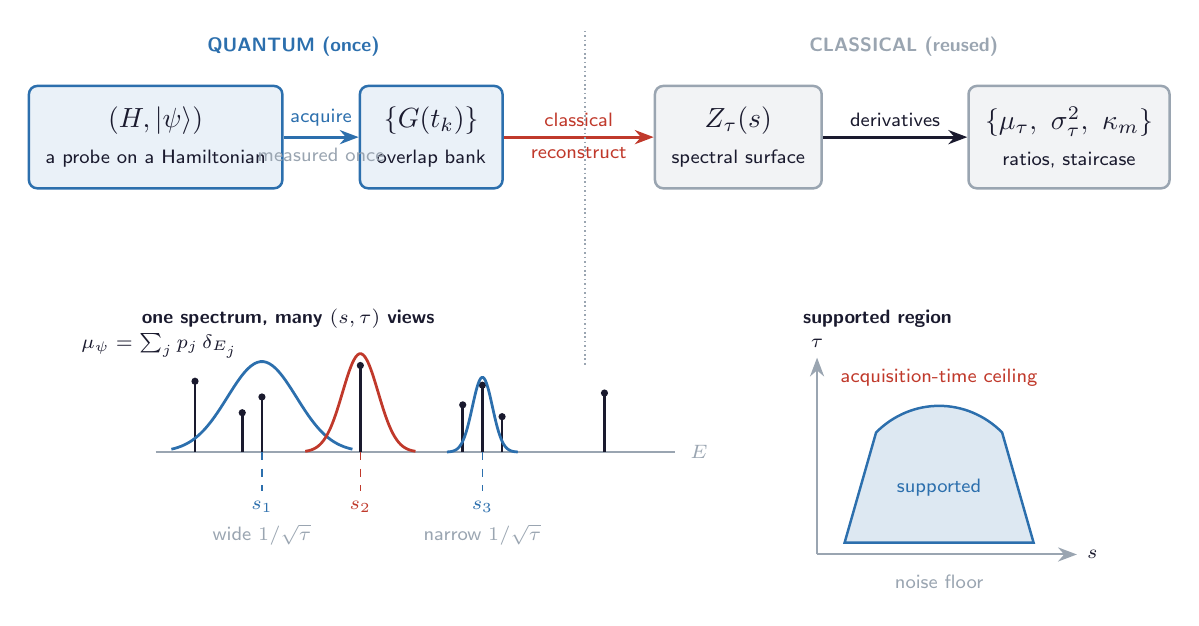
\begin{tikzpicture}[
  font=\sffamily,
  >={Stealth[length=2.4mm]},
  box/.style={rounded corners=3pt, line width=0.9pt, inner sep=6pt,
              align=center, text=ink, minimum height=13mm},
  qbox/.style={box, draw=phys, fill=physbg},
  cbox/.style={box, draw=faint, fill=inkbg},
  lab/.style={font=\scriptsize\sffamily, text=ink},
  flow/.style={->, line width=1pt},
]

% ===================== TOP ROW: the pipeline ==============================
\node[qbox] (src) at (0,0)
     {$(H,|\psi\rangle)$\\[1pt]{\scriptsize a probe on a Hamiltonian}};
\node[qbox] (bank) at (3.5,0)
     {$\{G(t_k)\}$\\[1pt]{\scriptsize overlap bank}};
\node[cbox] (surf) at (7.4,0)
     {$Z_\tau(s)$\\[1pt]{\scriptsize spectral surface}};
\node[cbox] (read) at (11.6,0)
     {$\{\mu_\tau,\ \sigma^2_\tau,\ \kappa_m\}$\\[1pt]{\scriptsize ratios, staircase}};

\draw[flow, phys] (src) -- node[lab, above, text=phys]{acquire}
                              node[lab, below, text=faint]{measured once} (bank);
\draw[flow, acc] (bank) -- node[lab, above, text=acc]{classical}
                            node[lab, below, text=acc]{reconstruct} (surf);
\draw[flow, ink] (surf) -- node[lab, above]{derivatives} (read);

% quantum / classical banners
\node[lab, text=phys, font=\scriptsize\bfseries\sffamily]
     at ($(src)!0.5!(bank) + (0,1.15)$) {QUANTUM (once)};
\node[lab, text=faint, font=\scriptsize\bfseries\sffamily]
     at ($(surf)!0.5!(read) + (0,1.15)$) {CLASSICAL (reused)};
\draw[faint, densely dotted, line width=0.6pt]
     ($(bank)!0.5!(surf) + (0,1.35)$) -- ($(bank)!0.5!(surf) + (0,-2.9)$);

% ===================== LOWER STRIP: one spectrum, many views ===============
\begin{scope}[shift={(0,-4.0)}, local bounding box=SPEC]
  % a generic spectral measure mu_psi: stems at eigenvalues
  \draw[faint, line width=0.6pt] (0,0) -- (6.6,0);
  \node[lab, text=faint] at (6.9,0) {$E$};
  \foreach \x/\h in {0.5/0.9, 1.1/0.5, 1.35/0.7, 2.6/1.1, 3.9/0.6, 4.15/0.85, 4.4/0.45, 5.7/0.75}{
     \draw[ink, line width=1pt] (\x,0) -- (\x,\h);
     \fill[ink] (\x,\h) circle (1.3pt);
  }
  \node[lab, text=ink] at (0.05,1.35) {$\mu_\psi=\sum_j p_j\,\delta_{E_j}$};

  % three Gaussian windows at locations s, differing resolutions 1/sqrt(tau)
  % wide window (small tau)
  \draw[phys, line width=1pt, domain=0.2:2.5, samples=60, smooth]
        plot (\x, {1.15*exp(-((\x-1.35)/0.62)^2)});
  \draw[phys, dashed, line width=0.5pt] (1.35,0) -- (1.35,-0.5)
        node[lab, below, text=phys]{$s_1$};
  % medium window
  \draw[acc, line width=1pt, domain=1.9:3.3, samples=60, smooth]
        plot (\x, {1.25*exp(-((\x-2.6)/0.32)^2)});
  \draw[acc, dashed, line width=0.5pt] (2.6,0) -- (2.6,-0.5)
        node[lab, below, text=acc]{$s_2$};
  % narrow window (large tau)
  \draw[phys, line width=1pt, domain=3.7:4.6, samples=60, smooth]
        plot (\x, {0.95*exp(-((\x-4.15)/0.18)^2)});
  \draw[phys, dashed, line width=0.5pt] (4.15,0) -- (4.15,-0.5)
        node[lab, below, text=phys]{$s_3$};

  \node[lab, text=faint, align=left] at (1.35,-1.05)
       {wide $1/\sqrt{\tau}$};
  \node[lab, text=faint, align=left] at (4.15,-1.05)
       {narrow $1/\sqrt{\tau}$};
\end{scope}
\node[lab, text=ink, font=\scriptsize\bfseries\sffamily, anchor=west]
     at (-0.3,-2.3) {one spectrum, many $(s,\tau)$ views};

% ===================== SUPPORTED (s,tau) REGION (lower right) ===============
\begin{scope}[shift={(8.4,-5.3)}, local bounding box=REG]
  \draw[->, faint, line width=0.7pt] (0,0) -- (3.3,0) node[lab, right, text=ink]{$s$};
  \draw[->, faint, line width=0.7pt] (0,0) -- (0,2.5) node[lab, above, text=ink]{$\tau$};
  % supported region: bounded above by acquisition time, on the flanks by noise
  \fill[phys, opacity=0.16]
     (0.35,0.15) -- (2.75,0.15) -- (2.35,1.55)
     .. controls (1.9,2.0) and (1.2,2.0) .. (0.75,1.55) -- cycle;
  \draw[phys, line width=0.9pt]
     (0.35,0.15) -- (2.75,0.15) -- (2.35,1.55)
     .. controls (1.9,2.0) and (1.2,2.0) .. (0.75,1.55) -- cycle;
  \node[lab, text=phys, align=center] at (1.55,0.85) {supported};
  \node[lab, text=acc, align=center] at (1.55,2.25)
       {\scriptsize acquisition-time ceiling};
  \node[lab, text=faint, align=center] at (1.55,-0.35)
       {\scriptsize noise floor};
\end{scope}
\node[lab, text=ink, font=\scriptsize\bfseries\sffamily, anchor=west]
     at (8.1,-2.3) {supported region};

\end{tikzpicture}
\end{document}
